\documentclass[11pt]{article}
\usepackage[T1]{fontenc}
\usepackage[a4paper,margin=25mm]{geometry}
\usepackage{amsmath,amssymb,amsthm}
\usepackage{graphicx}
\usepackage[hidelinks]{hyperref}
\usepackage{microtype}

\newtheorem{theorem}{Theorem}
\newtheorem{lemma}{Lemma}
\newcommand{\C}{\mathbb C}
\newcommand{\D}{\overline{\mathbb D}}
\newcommand{\DD}{D^{(1)}}
\newcommand{\norm}[1]{\lVert#1\rVert}
\newcommand{\abs}[1]{\lvert#1\rvert}

\setlength{\parindent}{0pt}
\setlength{\parskip}{0.6em}

\title{The Function $Q_X$ Is Not Local with Respect to\\
Connected Compact Neighbourhoods}
\author{Run \texttt{fa\_banach\_001} --- lane 14}
\date{11 August 2026}

\begin{document}
\maketitle

\begin{center}
\fbox{\parbox{0.91\textwidth}{
\textbf{Status: full counterexample to Open Question 8.}
There are a connected compact plane set $X$, a point $z_0\in X$, and a
connected compact neighbourhood $N$ of $z_0$ in $X$ such that
\[
 Q_N(z_0)=\infty
 \qquad\text{but}\qquad
 Q_X(z_0)=1.
\]
Indeed, $X$ may be the closed unit disk.  Thus the implication asked for by
Dales and Feinstein is false, even for a convex ambient set.
}}
\end{center}

\section{Source question}

For a connected compact plane set $Y$ and $z\in Y$, Dales and
Feinstein~\cite{source} define
\[
 Q_Y(z)=\sup\left\{
 \frac{\abs{f(z)-f(y)}}{\abs{z-y}}:
 y\in Y\setminus\{z\},\ f\in\DD(Y),\ \abs{f'}_Y\le1
 \right\}.
\]
Their Open Question~8 on arXiv PDF page~31 asks whether
$Q_N(z_0)=\infty$ for a connected compact neighbourhood $N$ of $z_0$ in
$X$ must imply $Q_X(z_0)=\infty$.

\begin{figure}[ht]
  \centering
  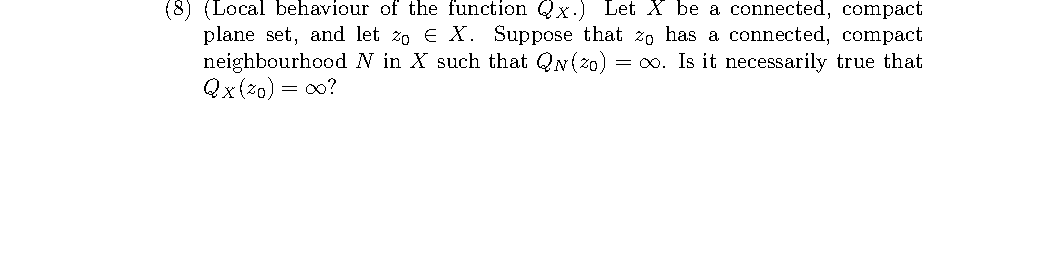
\includegraphics[width=0.94\textwidth]{figures/open_question_8.png}
  \caption{Open Question~8 on source PDF page~31.}
\end{figure}

\section{Counterexample}

\begin{theorem}\label{thm:main}
Let $X=\D$, let $z_0=0$, and let
$E=\{z\in\C:\abs z\le1/4\}$.  There is a non-rectifiable Jordan arc
$J\subset X$ with endpoints $q=1/4$ and $w=3/4$ such that
$J\cap E=\{q\}$.  For
\[
 N=E\cup J
\]
we have
\[
 Q_X(0)=1,\qquad Q_N(0)=\infty.
\]
In particular, the answer to Open Question~8 is no.
\end{theorem}

Such an arc is elementary to arrange: leave $q$ along the real segment to a
point outside $E$, then continue along a sufficiently small scaled Koch arc
ending at $w$.  The construction can be kept in a thin rectangle contained in
the open unit disk and disjoint from $E$ except at $q$.  Adding the initial
segment preserves the Jordan property and leaves the total length infinite.

\section{Idea of the proof}

The ambient disk has every straight segment available, so bounded derivative
forces the sharp Euclidean Lipschitz estimate and $Q_X(0)=1$.  The thin
neighbourhood $N$, however, contains a non-rectifiable arc.  A lemma already
proved in the source constructs functions on an arbitrarily long Jordan arc
whose derivative is uniformly bounded but whose endpoint oscillation is as
large as desired, with derivative zero at both endpoints.  The zero endpoint
derivative lets us patch each such function constantly across the small disk
$E$.  These functions belong to $\DD(N)$ but cannot arise by restriction from
the full disk.  This mismatch makes $Q_N(0)$ infinite while $Q_X(0)$ stays
minimal.

\section{Proof}

We use the following source result.

\begin{lemma}[Dales--Feinstein, Lemma 10.4]\label{lem:longarc}
Let $a,b\in\C$, let $A>0$, and let $\gamma$ be a Jordan path from $a$ to $b$
whose length is greater than $A$ (infinite length is allowed).  Then there is
$h\in\DD(\gamma^*)$ such that
\[
 0<\abs{h'}_{\gamma^*}\le3,
 \qquad h'(a)=h'(b)=0,
 \qquad \abs{h(a)-h(b)}>A/2.
\]
\end{lemma}

First compute $Q_X(0)$.  Let $f\in\DD(X)$ with $\abs{f'}_X\le1$ and let
$u\in X$.  The straight segment $t\mapsto tu$ lies in $X$.  The one-variable
fundamental theorem of calculus, applied to $t\mapsto f(tu)$, gives
\[
 \abs{f(u)-f(0)}
 \le \int_0^1 \abs{u f'(tu)}\,dt
 \le \abs u.
\]
Thus $Q_X(0)\le1$.  The coordinate function $f(z)=z$ gives equality for every
$u\ne0$, hence
\[
 Q_X(0)=1.\tag{1}
\]

We now prove that $Q_N(0)=\infty$.  Fix $A>0$.  Since $J$ has infinite
length, Lemma~\ref{lem:longarc} gives $h_A\in\DD(J)$ such that
\[
 \abs{h_A'}_J\le3,\qquad h_A'(q)=0,\qquad
 \abs{h_A(q)-h_A(w)}>A/2.
\]
Define $F_A:N\to\C$ by
\[
 F_A(z)=
 \begin{cases}
   h_A(q),&z\in E,\\
   h_A(z),&z\in J.
 \end{cases}
\]
This is well defined because $E\cap J=\{q\}$.  It belongs to $\DD(N)$.
Away from $q$ this follows separately on the two compact pieces.  At $q$, the
difference quotient is identically zero along $E$ and converges to
$h_A'(q)=0$ along $J$; hence $F_A'(q)=0$.  The same two-piece observation,
together with continuity of $h_A'$ and $h_A'(q)=0$, shows that $F_A'$ is
continuous on $N$.  Therefore
\[
 \abs{F_A'}_N\le3.
\]

Set $G_A=F_A/3$.  This is an admissible test function in the definition of
$Q_N(0)$, and $G_A(0)=h_A(q)/3$.  Consequently
\[
 Q_N(0)
 \ge \frac{\abs{G_A(0)-G_A(w)}}{\abs w}
 >\frac{A}{6\abs w}.
\]
Since $A$ is arbitrary and $w=3/4$ is fixed,
\[
 Q_N(0)=\infty.\tag{2}
\]
The set $N$ is compact and connected.  It is a neighbourhood of $0$ in $X$
because it contains the relative open set
$X\cap\{z:\abs z<1/4\}$.  Equations (1)--(2) therefore give exactly the
counterexample asserted in Theorem~\ref{thm:main}.

\section{Strength and scope}

The example uses no pathology in the ambient geometry: $X$ is convex,
pointwise regular, polynomially convex, and has nonempty interior.  The value
$Q_X(0)=1$ is the smallest possible value.  The construction is also robust:
any convex compact set containing a small convex core and an attached
non-rectifiable Jordan arc gives the same phenomenon after rescaling.

The word ``neighbourhood'' is used in its standard topological sense: $N$
contains a relatively open neighbourhood of $z_0$ in $X$.  No claim is made
for stronger variants in which $N$ is required, for example, to be the closure
of a relatively open connected set.

The run's registry, solution, attempt, and proof-gap indexes were searched by
arXiv id, title, ``local behaviour $Q_X$,'' ``$Q_N(z_0)$,'' ``compact
neighbourhood,'' and ``non-rectifiable Jordan arc.''  Exact-phrase and topic
searches found no later resolution of Question~8.  The only imported
ingredient is source Lemma~10.4, stated in full above; the attachment and both
$Q$ computations are new deductions.

\begin{thebibliography}{9}
\bibitem{source}
H. G. Dales and J. F. Feinstein,
\emph{Normed algebras of differentiable functions on compact plane sets},
Indian J. Pure Appl. Math. \textbf{41} (2010), 153--187;
arXiv:1501.03986.
\end{thebibliography}

\end{document}
